\begingroup
\centering
\captionsetup{type=figure}
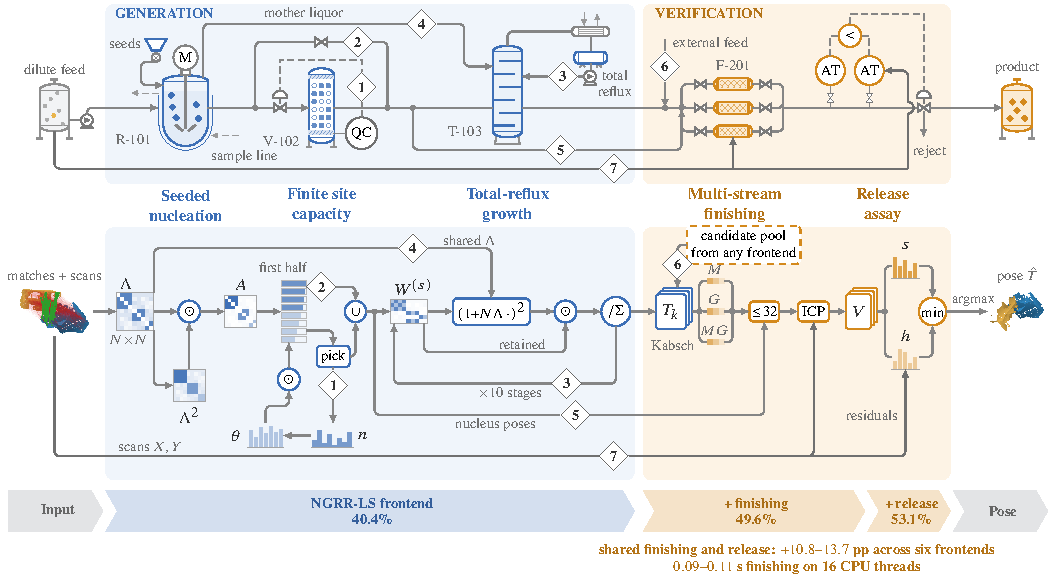
\includegraphics[width=\textwidth]{shared/figures/fig_dataflow.pdf}
\captionof{figure}{The chemical process (top) and registration data flow (bottom). NGRR-LS supplies one candidate pool, while the dashed entry makes the finishing and release backend available to any frontend. The compatibility matrix $\Lambda$ is used to generate hypotheses, which finishing turns into a refined pool $V$. Its candidates are evaluated by support $s$ and residual shape $h$. Release selects $\arg\max_k\min(s_k,h_k)$, corresponding to the low-signal selector over two analyzers. Diamonds 1--7 identify corresponding connections, including 3 for growth stages and total reflux and 7 for scans and the sample line. The bottom strip reports \ls{} recall on 3DLoMatch+FPFH after each stage. The refined-pool ceiling is 59.2\%. Scans are real, while matrices and equipment are schematic.}
\label{fig:flowsheet}
\endgroup%
